%
% File acl2014.tex
%
% Contact: koller@ling.uni-potsdam.de, yusuke@nii.ac.jp
%%
%% Based on the style files for ACL-2013, which were, in turn,
%% Based on the style files for ACL-2012, which were, in turn,
%% based on the style files for ACL-2011, which were, in turn, 
%% based on the style files for ACL-2010, which were, in turn, 
%% based on the style files for ACL-IJCNLP-2009, which were, in turn,
%% based on the style files for EACL-2009 and IJCNLP-2008...

%% Based on the style files for EACL 2006 by 
%%e.agirre@ehu.es or Sergi.Balari@uab.es
%% and that of ACL 08 by Joakim Nivre and Noah Smith

\documentclass[11pt]{article}
\usepackage{acl2014}
\usepackage{times}
\usepackage{url}
\usepackage{latexsym}
\usepackage{graphicx}
\usepackage[labelfont=bf]{caption}
\usepackage{xcolor}

%\setlength\titlebox{5cm}

% You can expand the titlebox if you need extra space
% to show all the authors. Please do not make the titlebox
% smaller than 5cm (the original size); we will check this
% in the camera-ready version and ask you to change it back.


\title{Ling 573 Project: Multi-Document Summarization}

\author{Emma Bateman \\
  {\tt ebateman@uw.edu} \\\And
  John Dodson \\
  {\tt jrdodson@uw.edu} \\\And
  Charlie Guo \\
  {\tt qcg@uw.edu}
  }

\date{}

\begin{document}
\maketitle
\begin{abstract}
We describe an unsupervised multi-document summarization system. Given a corpus, salient sentences are selected through the TextRank algorithm and then re-ordered using a local coherence algorithm for modeling entity distributions across the text. The ordered result set is then compressed using either rule-based or machine learning techniques. The system is divided into three components for ranking salient sentences, logical ordering, and result compression. We evaluate our system on the AQUAINT, AQUAINT-2, and Gigaword corpora.
\end{abstract}

\section{Introduction}

Multi-document summarization systems seek to aggregate collections of text documents and condense their content to provide cohesive summaries. Traditional approaches to summarization fall into two distinct categories: abstractive and extractive. Abstractive techniques are categorized based on their ability to generate novel summary content, in contrast with extractive approaches which select significant content directly from the source documents. In this work, we present an unsupervised system for extractive multi-document summarization over a benchmark dataset. The system is centered around the TextRank algorithm, which is a graph-based technique to identify and rank the most salient sentences in the input documents. We evaluate our system on the AQUAINT, AQUAINT-2, and Gigaword corpora, with average ROUGE-1 and ROUGE-2 F-scores of $0.28385$ and $0.07365$, respectively. 

This report is structured as follows: Section 2 provides an overview of our system and its components, including a brief description of the datasets used to train and evaluate the experiment; section 3 details our approach to generating summaries using TextRank, entity-grid representations, and compression techniques; section 4 presents result metrics; section 5 is a discussion and error analysis; and section 6 concludes.

\section{System Overview}
The system is divided into three primary components: a graph-based content selector, an ordering algorithm, and a compression algorithm. The content selector is responsible for ingesting a schema file which details one or more document clusters in the AQUAINT and Gigaword datasets. The selector identifies which documents belong together in a cluster and then ingests those documents as plain text. The system extracts feature vectors from each sentence by computing word frequencies. The feature vectors are given as input to the  TextRank algorithm to sort vectors by salience. Sentences are selected and compressed in order of salience until the summary surpasses the word limit (100 words) at which point the last sentence is discarded. Sentences are ordered by one of of two methods: they are either fed through an entity-grid based algorithm, or ranked by the shortest path between their feature vectors. The logically ordered sentences are further compressed using either a rule-based algorithm or a MaxEnt model trained to compress text.

\subsection{Architecture}
\begin{figure}
  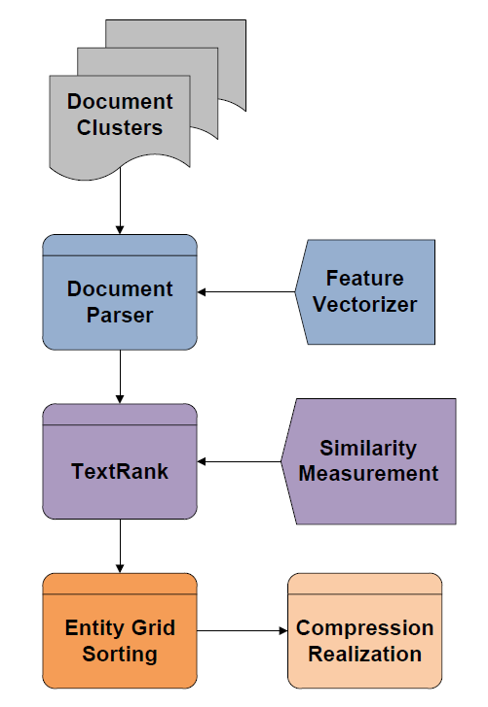
\includegraphics[width=.9\linewidth,height=.25\textheight,keepaspectratio]{arch_final.png}
  \caption{Multi-document summarization system architecture.}
  \label{fig:arch}
\end{figure}

Figure \ref{fig:arch} provides an illustration of the existing system architecture.

\subsection{Datasets}
We use the AQUAINT (Advanced Question-Answering for Intelligence) and AQUAINT-2 corpora to provide input to our system. Both datasets are composed of English newswire texts. For the multi-document summarization task, we leverage a corresponding schema file which defines one or more document-topic clusters. For evaluation, we use a subset of the Gigaword dataset.

\section{Approach}

This section details the main components of the working system.

\subsection{Content Selection}
The ingest processor for the system consumes one or more documents associated with a cluster identifier. These SGML documents are converted to plain text and represented as a single monolithic text string. After ingest is complete, the system will maintain one text representation per document cluster.

The system uses BeautifulSoup to perform most of its SGML and XML parsing. For a given input file, the ingest processor identifies clusters and their associated documents by finding document IDs which correspond to AQUAINT SGML files. The system then loads the corresponding SGML files and pefrorms traversal using BeautifulSoup to find the appropriate blocks of text.
\subsubsection{Feature Vectors}
The feature extraction component takes the plain text representation and tokenizes it into individual sentences using Python's Natural Language Toolkit (NLTK). NLTK is used to remove common stopwords from each sentence. Feature vectors are generated in two steps: firstly, the component identifies a comprehensive vocabulary for the cluster; and secondly, a frequency vector is created based on the token frequencies in the given sentence. 

The output of this component is an $N$ x $V$ matrix, where $N$ is the total number of sentences in the cluster and $V$ is the size of the vocabulary. 
\subsubsection{TextRank}
Our system uses TextRank to compute saliency scores for each sentence in the cluster and subsequently rank them according to significance. The TextRank algorithm constructs a graphical representation of textual features, where a given textual feature is represented as a vertex in the graph. The algorithm assigns a significance score to each vertex based on inbound edge weighting.

The authors of the TextRank algorithm formally define a graph as a tuple $G = (V,E)$, where $V = \{v_1, v_2, ... v_n\}$ is the set of vertices in the graph and $E$ is a set of edges and a subset of $V$ x $V$. TextRank is inspired by PageRank and computes the score for some vertex $V_i$ similarly to the original algorithm:
\begin{center}
    $S(V_i) = (1 - d) + d * \sum_{j \in In(V_i)} \frac{1}{|Out(V_j)|}S(V_j)$
\end{center}
$In(V_i)$ represents all inbound connections to vertex $V_i$, and $Out(V_j)$ represents outbound connections from vertex $V_j$. The authors use $d$ as a damping factor set between $0$ and $1$, which effectively biases the calculation. The original PageRank algorithm defaults this factor to $0.85$, and in our system we maintain this defaulted value.

In applying TextRank to sentence processing, we compute a pairwise similarity matrix of size $N$ x $N$, where $N$ is the total number of sentences in the cluster. The similarity between $N_i$ and $N_j$ becomes the edge weight which connects those two vertices in the graph. We use cosine similarity as our distance measurement.

After the TextRank algorithm converges, the algorithm returns the top K sentences as the cluster summary. Each summary contains 100 words maximum. The system maintains a 
reference to the original sentences, and uses the original text as output.

\subsubsection{Redundancy}
In our earlier system, we encountered significant amounts of redundancy, including repeated sentences. In one case, a sentence appeared in a summary three times in a row. 

\begin{quote}
``The nation deserves and I will select a Supreme Court justice that Americans can be proud of," Bush said.\\
``The nation deserves and I will select a Supreme Court Justice that Americans can be proud of," Bush said.\\
``The nation deserves and I will select a Supreme Court justice that Americans can be proud of," Bush said.\\
Sandra Day O'Connor, the first  woman ever appointed to the US Supreme Court, said Friday that she is retiring, giving US president George W. Bush his first  opportunity to appoint a justice.
\end{quote}

We fixed this issue by modifying the TextRank algorithm. At each iteration, until enough sentences have been selected to complete the summary, the most salient sentence is extracted. Then, the corresponding feature vector is subtracted from the rest of the matrix, disadvantaging sentences with a high level to similarity to the selected sentence. Finally, the similarity algorithm is rerun before the next sentence is selected.\\

\subsection{Information Ordering}
The system uses an entity-based modeling approach to improve summary coherence and provide a more logical ordering of the sentences in each summary. Our approach is inspired by the entity grid mechanism introduced in Barzilay and Lapata 2008, wherein the authors describe a local coherence algorithm centered around entity transitions. Our algorithm models the distribution of entities across the top outputs of TextRank, which means the input data is fundamentally small. We make the assumption that the input sentences naturally contain local coherence after applying TextRank. 

\subsubsection{Extracting Grammatical Roles}
The authors of the original algorithm exploit several factors in their entity representations, namely, coreference resolution, grammatical roles, and saliency. Our system only uses grammatical function in determining entity types. We use the Stanford CoreNLP toolkit to generate dependency parses over each input sentence. Subject and object relations are extracted from the parse tree and used to model entity transitions. We provide weights for entities with subject, object, and alternate relation categories.

\subsubsection{Entity Grid Representation}
Following the conventions established in Barzilay and Lapata 2008, we use the grammatical roles described in Section 3.2.1 to denote types of discourse entities. After generating dependency parses and compiling the set of unique entities in the input corpus, we compile a table representation of size $N$ x $M$, where $N$ is the total number of sentences in the input corpus and $M$ is the total number of unique entities extracted from that corpus. In our system $N$ is reasonably small.

The entity grid is populated with weight values corresponding to the grammatical function of an entity in a given sentence, where a table entry $E_{i,j}$ is weighted depending on the grammatical role of entity $j$ in sentence $i$. 


\subsubsection{Shortest Path}
The shortest path ordering algorithm orders the sentences by solving the traveling salesman problem for the feature vectors of the selected sentences. 

The distances between vectors are calculated using cosine similarity.

The sentences are output in the order of the shortest path, starting with the most salient of the two endpoints.

\subsection{Compression}
This section discusses the sentence compression modules for proper content realization.

\subsubsection{Rule-based compression}
A rule-based compression is implemented in our system which shortens each sentence by parsing each sentence and then removing less important syntactic component such as PP and DT. Here is an example of a shortened sentence in our system output:
\\
\fbox{\begin{minipage}{17em}
\small {

Senior Palestinian official Yasser Abed Rabbo denied on Tuesday reports saying that Palestinian leader Yasser Arafat has died {\color{gray}in a French hospital}.

} \\
\end{minipage}}
\\

The system leverages a named entity recognition capability to identify and simplify individual person mentions when a name is referenced multiple times. For example:
\\

\fbox{\begin{minipage}{17em}
\small {
\par \noindent 
Senior Palestinian official  denied reports saying that Palestinian leader {\bfseries Yasser Arafat} has died. 
\newline \par \noindent
As {\bfseries Arafat} had struggled for life, there has been wild guess as to ...
\newline \par \noindent
French foreign minister told LCI television that {\bfseries Arafat} was alive but that ...
\newline \par \noindent
Palestinian leader {\color{gray}Yasser} {\bfseries Arafat} would be buried at his headquarters in the West Bank town of Ramallah.
}
\end{minipage}}
\\

We did not exhaust all possible syntactic components. This is discussed further in subsequent sections.

\subsubsection{Model-based compression}

Our model-based compression algorithm is based on the work of Wang et al (2013).

We began by training a MaxEnt model on hand-annotated compression data from Clarke and Lapata (2008). The training data was downloaded from \url{https://www.jamesclarke.net/research/resources}. We used 1000 sentences from the Broadcast News Compression Corpus.

The feature vectors used for training were many of the same features used in Wang et al, including:
\begin{itemize}
\item all leaves fall within first 3 tokens?
\item all leaves fall within last 3 tokens?
\item subsumes first 3 tokens?
\item subsumes last 3 tokens?
\item contains words longer than 10 letters?
\item subsumes only one leaf?
\item subsumes entire sentence?
\item contains capitalization?
\item contains all caps word?
\item contains negation?
\item contains stopwords?
\item falls within parenthetical?
\item contains lead adverbial?
\item contains relative clause?
\item contains lead prepositional clause?
\item depth of node
\item node label
\item left sibling node label
\item right sibling node label
\item left sibling node label of parent
\item right sibling node label of parent
\end{itemize}

We formulated the problem space for each sentence as the possible sequences of ``keep" and ``delete" labels for each node of the syntax tree. We then performed a heuristic search of the problem space with the trained MaxEnt model as the scoring function. At each node, our algorithm performs search recursively on each child node, then returns the 5 highest scoring sequences found using those results. Of the five sequences discovered by running search on the head node, the highest scoring one is used to compress the sentence.

\subsection{Baseline System}
The baseline for this experiment is a system with each aforementioned component except the compression algorithms. In theory, this baseline still generates ordered salient results but disregards human readability. The baseline is evaluated on the development corpus comprised of AQUAINT and AQUAINT-2 data.

\section{Results}
We present result metrics for both ROUGE-1 and ROUGE-2 over the development and evaluation corpora. In addition, we provide human evaluations for six generated summaries. 

\subsection{ROUGE scores}
\textbf{Table 1} and \textbf{Table 2} present ROUGE-1 and ROUGE-2 metrics for development and evaluation data. For the development set, the best reported  ROUGE-1 F1 score is given by the baseline algorithm. The reduced scores in the updated system are likely due to the compression component, which focuses on readability. Similarly, for the ROUGE-2 scores, the baseline algorithm gives the best recall, precision, and F1 metrics.

\begin{table*}[h]
\begin{tabular}{|p{4.3cm}||p{1.735cm}|p{1.78cm}|p{1.735cm}|p{1.735cm}|p{1.78cm}|p{1.735cm}| }
 \hline
 \multicolumn{7}{|c|}{Development set ROUGE-1 and ROUGE-2 scores} \\
 \hline
 \textbf{Algorithm} & \textbf{ROUGE-1 Recall} & \textbf{ROUGE-1 Precision} & \textbf{ROUGE-1 F1} & \textbf{ROUGE-2 Recall} & \textbf{ROUGE-2 Precision} & \textbf{ROUGE-2 F1}\\
 \hline
Baseline algorithm & 0.21358 & \textbf{0.27155} & \textbf{0.23732} & \textbf{0.05335} & \textbf{0.06814} & \textbf{0.05937} \\ 
Entity grid, rule-based & 0.21643 & 0.23487 & 0.22322 & 0.05036 & 0.05311 & 0.05133 \\
Shortest path, rule-based & \textbf{0.21865} & 0.23280 & 0.22400 & 0.05054 & 0.05282 & 0.05136 \\
Entity grid, model-based & 0.20716 & 0.27003 & 0.23264 & 0.04610 & 0.05970 & 0.05169 \\
Shortest path, model-based & 0.20730 & 0.27023 & 0.23280 & 0.04586 & 0.06043 & 0.05173 \\
\hline
\end{tabular}
\caption{Evaluation metrics on AQUAINT data}
\label{tab:dev} 
\end{table*}

\begin{table*}[h]
\begin{tabular}{|p{4.3cm}||p{1.735cm}|p{1.78cm}|p{1.735cm}|p{1.735cm}|p{1.78cm}|p{1.735cm}| }
 \hline
 \multicolumn{7}{|c|}{Evaluation set ROUGE-1 and ROUGE-2 scores} \\
 \hline
 \textbf{Algorithm} & \textbf{ROUGE-1 Recall} & \textbf{ROUGE-1 Precision} & \textbf{ROUGE-1 F1} & \textbf{ROUGE-2 Recall} & \textbf{ROUGE-2 Precision} & \textbf{ROUGE-2 F1}\\
 \hline
Entity grid, rule-based & 0.25371 & 0.27168 & 0.26009 & 0.06173 & 0.06545 & 0.06281 \\
Shortest path, rule-based & 0.25628 & 0.26949 & 0.26154 & 0.06235 & 0.06441 & 0.06305 \\
Entity grid, model-based & \textbf{0.25656} & \textbf{0.32682} & \textbf{0.28385} & \textbf{0.06695} & \textbf{0.08390} & \textbf{0.07365} \\
Shortest path, model-based & 0.24993 & 0.31408 & 0.27512 & 0.06276 & 0.07798 & 0.06882 \\
\hline
\end{tabular}
\caption{Evaluation metrics on Gigaword data}
\label{tab:dev} 
\end{table*}

\subsection{Human Evaluation}
Readability is an important aspect of document summarization that is not represented by ROUGE scores. \textbf{Table 3} shows human eval scores for six of our summaries based on ratings given by 4 annotators on a scale from 1 to 5.

\begin{table*}[h]
	\centering
	\begin{tabular}{|c|p{1cm}|p{1cm}|p{1cm}|p{1cm}|p{1cm}|}
	\hline
		\textbf{Topic} & \multicolumn{4}{|c|}{\textbf{Individual annotator scores}} & \textbf{mean}\\
	\hline
	Plane crash Indonesia & 2 & 3 & 4 & 3 & 3.0\\
	\hline
	Tuna overfishing & 2 & 2 & 3 & 4 & 2.75\\
	\hline
	China food safety & 3 & 1 & 2 & 2 & 2.0\\
	\hline
	Cyclone Sidr & 2 & 2 & 3 & 3 & 2.5\\
	\hline
	Dimona attack & 2 & 2 & 3 & 4 & 2.75 \\
	\hline
	Sichuan earthquake & 2 & 2 & 3 & 2 & 2.25\\
	\hline
\end{tabular}
\caption{Human evaluation of 6 summaries}
\label{tab:dev}
\end{table*}

\section{Discussion \& Error Analysis}

By visually checking results from both development and evaluation data, we did identify several of issues related to compression and content realization. One is the loss of grammaticality after compression, which happened on many cases of incomplete removal of PP, which can be illustrated by the following example:
\\

\fbox{\begin{minipage}{17em}
\small {

The death toll {\bfseries from the} that struck the coastline {\bfseries near the} of Aitape in the province Friday night, was announced 64 and people were missing.

}
\end{minipage}}
\\ 

Secondly, pronouns occasionally appear without an antecedent. This is due to the lack of support for anaphora resolution. 
\\

\fbox{\begin{minipage}{17em}
\small {
\par \noindent 
{\bfseries He} said that the company did not ...
\newline \par \noindent
{\bfseries He} estimated that ... 
}
\end{minipage}}
\\

Beyond the rule-based module, handcrafting additional features for the MaxEnt implementation is another potential area of improvement. Given that the model-based compression system outperformed every other system configuration for the evaluation data, further feature engineering for the model training data could potentially yield improved metrics.

Other minor issues such as missing and mismatching punctuations were also identified. All these issues affected the readability of the summaries.


\section{Conclusion}
 We have described an unsupervised system for generating single summaries over multiple documents. The system generates feature vectors per sentence by computing word frequencies, and then provides those frequency vectors as input to the TextRank algorithm. The algorithm is able to identify significant lines of text in a single pass. We take the top K sentences as the corresponding summary, up to 100 words max per summary. The system leverages an entity grid algorithm for intelligent sentence ordering, and cleans the output text through one of two compression implementations.

% include your own bib file like this:
%\bibliographystyle{acl}
%\bibliography{acl2014}
\begin{thebibliography}{}

\bibitem{textrank04}
	Rada Mihalcea and Paul Tarau,
	\textit{TextRank: Bringing Order into Texts},
	Proceedings of the 2004 Conference on Empirical Methods in Natural Language Processing,
	2004.

\bibitem{entitygrid08}
    Regina Barzilay and Mirella Lapata,
    \textit{Modeling Local Coherence: An Entity-Based Approach}
    Computational Linguistics, 
    2008
\bibitem{wang13}
	Lu Wang et al,
	\textit{A Sentence Compression Based Framework to Query-Focused Multi-Document Summarization},
	Proceedings of the 51st Annual Meeting of the Association for Computational Linguistics, pages 1384-1394,
	2013
\bibitem{clarke08}
	James Clarke and Mirella Lapata,
	\textit{Global Inferece for Sentence Compression: An Integer Linear Programming Approach},
	Journal of Artificial Intelligence Research vol 31, pages 399-429,
	2008

\end{thebibliography}

\end{document}
